%! TEX root = ./thesis.tex
\chapter{Grundlagen}\label{chap:prelim}

Dieses Kapitel legt die Grundlagen für die folgenden Kapitel fest. Abschnitt~\ref{sec:notation} erläutert mathematische Notationen für diese Arbeit. Abschnitt~\ref{sec:prelim-machines} spezifiziert das Maschinenmodell.  Abschnitt~\ref{sec:prelim-klassen} wiederholt einige Standarddefinitionen aus der Komplexitätstheorie. Abschnitt~\ref{sec:prelim-orakel} setzt das hier verwendete Verständnis von Relativierungen fest. Abschließend geht Abschnitt~\ref{sec:prelim-ps} kurz auf Beweissysteme im Sinne von \textcite{cook_relative_1979} ein.

\section{Notation}\label{sec:notation}

Sei $\Sigma$ das standardmäßige Alphabet mit $\Sigma=\{0,1\}$. Elemente von $\Sigma^*$ nennen wir (endliche) \emph{Wörter}, sind also endliche Sequenzen von Zeichen aus $\Sigma$. Die Menge $\Sigma^\omega$ entspricht der Menge der $\omega$-unendlichen Wörter. Teilmengen von $\Sigma^*$ nennen wir auch Sprachen. Wir bezeichnen die Länge eines Wortes $w\in\Sigma^*$ mit $|w|$. Das leere Wort bezeichnen wir mit $\epsilon$. Das $i$-te Zeichen eines Wortes $w\in\Sigma^*\cup\Sigma^\omega$ für $0\leq i< |w|$ identifizieren wir mit $w[i]$. 
Falls $w$ ein (echter) Präfix von $v$ ist dann schreiben wir $w \sqsubseteq v$ (bzw. $w\sqsubsetneq v$).
Gelegentlich schreiben wir auch $\Sigma^{\leq n}$ für die Menge $\{ w\in\Sigma^* \mid |w|\leq n\}$. 
In manchen Fällen identifizieren wir Mengen $A\subseteq\mathbb N$ mit ihrem charakteristischem $\omega$-Wort aus $\Sigma^\omega$, wobei $A=a_0a_1a_2\cdots$, alle $a_i\in\Sigma$ und $i\in A$ genau dann wenn $a_i=1$.
Heißt, es gilt $A[i] = 1$ genau dann wenn $i\in A$.

Die Menge aller natürlichen (nicht-negativen) Zahlen wird mit $\mathbb N$ bezeichnet. Die leere Menge notieren wir wie üblich als $\emptyset$. Die Kardinalität einer Menge $A$ notieren wir wie üblich als $|A|$. 
%Analog definieren wir $A^{<n}, A^{=n}$, usw. 
Außerdem bezeichnet $\ell(A)\defeq\sum_{w\in A} |w|$. Für solche Teilmengen $A$ von $\Sigma^*$ verstehen wir das Komplement $\overline{A}$ als $\Sigma^*-A$.
Wir sagen, dass zwei Mengen $A, B$ \emph{auf Menge $D$ übereinstimmen} wenn $x\in A$ genau dann wenn $x\in B$ für alle $x\in D$, bzw. äquivalent dazu $A\cap D= B\cap D$.

Für zwei Mengen $A, B\subseteq\Sigma^*$ bezeichnet der \emph{Join} $A\oplus B$ die Menge
\[ A\oplus B \defeq \{0a\mid a\in A\} \cup \{1b\mid b\in B\}. \]


\subsection*{Relationen und Funktionen}

Zweistellige bzw. binäre Relationen $R\subseteq A\times B$ können wir mit den üblichen Eigenschaften beschreiben: die Relation $R$ ist
\begin{itemize}[midpenalty=0]
    \item \emph{(links-)total} wenn jedes Element aus $A$ mit mindestens einem Element aus $B$ reliert,
    \item \emph{rechtstotal} bzw. \emph{surjektiv} wenn jedes Element aus $B$ mit mindestens einem Element aus $A$ reliert,
    \item \emph{linkseindeutig} bzw. \emph{injektiv} wenn jedes Element aus $B$ mit höchstens einem Element aus $A$ reliert,
    \item \emph{(rechts-)eindeutig} bzw. \emph{funktional} wenn jedes Element aus $A$ mit höchstens einem Element aus $B$ reliert,
    \item \emph{bijektiv} wenn jedes Element aus $B$ mit genau einem Element aus $A$ reliert, also genau dann wenn $R$ surjektiv und injektiv ist.
\end{itemize}
Binäre Relationen nennen wir eine (partielle) \emph{Funktion} wenn diese Relation funktional ist. Eine Funktion sei im Folgenden also im Allgemeinen nicht total. Sollte (Links-)Totalität explizit gefordert sein, sprechen wir von \emph{totalen Funktionen}.
%Beachte, dass eine totale bijektive Funktion $A\to B$ einen Mengenisomorphismus zwischen $A$ und $B$ bildet.
Binäre Relationen über Wörtern aus $\Sigma^*$, welche nicht unbedingt Funktionen sein müssen, verstehen wir manchmal auch aus historischen Gründen als (partielle) Multifunktionen, dem Begriff der „\emph{partial multivalued function}“ nachempfunden.

Für eine binäre Relation $R\subseteq A \times B$ schreiben wir $\Proj(R)$ für die Menge $\{ x\mid (x,y)\in R \}$. 
Für ein Element $x\in A$ schreiben wir $\fset{}R(x)=\{ y\mid (x,y)\in R \}$ für die Bildmenge von $x$ auf $R$
Manchmal werden wir binäre Relationen auch über die Spezifikation der jeweiligen Bildmengen definieren, also z.B. $Q\subseteq\mathbb N\times\mathbb N$, $\fset{}Q(n) \defeq \{ 0, 1, \dots, n\}$ schreiben um die Relation $Q=\{ (a,b)\mid b\leq a \}$ zu definieren.
%Für ein Wort $x\in\Sigma^*$ schreiben wir $R(x)= \{ y\mid (x,y)\in R \}$ für die Bildmenge von $x$ auf $R$. 
Falls $f$ eine Funktion bzw. funktional ist, meinen wir mit $f(x)$ wie üblich das \emph{Bildelement} der Funktion $f$, und nicht die \emph{Bildmenge}. 
%Es gilt also in diesem Fall $\fset{}f(x)=\{f(x)\}$.



Für eine Funktion $f$ bezeichnen wir die Urbild- bzw. Bildmenge (\emph{domain} und \emph{image}) mit $\dom(f)$ und $\img(f)$. (Beachte dass $\Proj(f)=\dom(f)$. Wir führen diese Unterscheidung nur wegen den Gewohnheiten dieser zwei Notationen ein.) Ist $f$ eine Funktion, dann bezeichnen wir mit $f^{-1}$ dessen binäre Umkehrrelation. Beobachte dass $f^{-1}$ funktional ist, wenn $f$ injektiv ist. Ist $f$ zusätzlich surjektiv, dann ist die Umkehrfunktion $f^{-1}$ eine totale Funktion.

Eine Funktion $f\colon\Sigma^*\to\Sigma^*$ nennen wir \emph{verlängernd} wenn $|f(x)|\geq |x|$ für alle $x\in\dom(f)$.
Wir nennen $f$ \emph{polynomiell längenbeschränkt} wenn ein Polynom $p$ existiert sodass $|f(x)|\leq p(|x|)$ für alle $x\in\dom(f)$.
Wir nennen $f$ \emph{ehrlich} wenn ein Polynom $q$ existiert sodass $q(|f(x)|)\geq |x|$ für alle $x\in\dom(f)$.
Manchmal übertragen wir diese Begrifflichkeiten auf allgemeine binäre Relationen, und sprechen z.B. von polynomiell längenbeschränkten Relationen $R$ wenn $|y|\leq p(|x|)$ für alle $(x,y)\in R$.

Im Folgenden definieren wir noch den Begriff der \emph{Verfeinerung} auf Multifunktionen. Seien $F, G$ zwei Multifunktionen. Wir nennen $G$ eine \emph{Verfeinerung} von $F$ wenn $\Proj(F)=\Proj(G)$ und $\fset{}G(x)\subseteq \fset{}F(x)$ für alle $x\in\Proj(F)$ (bzw. äquivalent $\in \Proj(G)$).
Ist $F$ eine Multifunktion, und $\mathcal G$ eine Klasse von Multifunktion, schreiben wir $F\inc \mathcal G$ wenn $\mathcal G$ eine Verfeinerung $G\in\mathcal G$ von $F$ enthält.
Für zwei Klassen $\mathcal F, \mathcal G$ von Multifunktionen schreiben wir $\mathcal F \subseteqc \mathcal G$ falls für jede Multifunktion $F\in\mathcal F$ auch $F\inc \mathcal G$ gilt.

\subsection*{Codierungen, Identifikation von Zahlen und Wörtern}

Die endlichen Wörter $\Sigma^*$ können über ihre quasi-lexikographischen Ordnung $\prec_\mathrm{lex}$ linear geordnet werden. Diese ist eindeutig definiert indem wir $0\prec_\mathrm{lex} 1$ fordern. Unter dieser Definition existiert ein Ordnungsisomorphismus zwischen $(\Sigma^*,\prec_\mathrm{lex})$ und $(\mathbb N, <)$, welcher insbesondere eine totale bijektive Abbildung zwischen $\Sigma^*$ und $\mathbb N$ induziert, die sowohl in Polynomialzeit berechenbar als auch invertiertbar ist. (Eine solcher Isomorphismus wird zum Beispiel durch eine dyadische Codierung realisiert.) Durch diese Identifikation können wir Wörter aus $\Sigma^*$ als Zahlen aus $\mathbb N$ behandeln und umgekehrt. Es können also auch Notationen, Beziehungen und Operationen für $\Sigma^*$ auf $\mathbb N$ übertragen werden und umgekehrt. Insbesondere können wir dann von einer Länge $|n|$ des Wortes sprechen, welches von $n\in\mathbb N$ repräsentiert wird. Insbesondere meint dieser Ausdruck nicht den Betrag von $n$. Ebenso bezeichnet die Ordnung $\leq$ sowohl die Kleiner-oder-gleich-Ordnung auf den natürlichen Zahlen als auch der quasi-lexikographischen Ordnung $\preceq_\mathrm{lex}$ auf den endlichen Wörtern. Diese Übereinstimmung ist nach den Eigenschaften des Ordnungsisomorphismus auch kompatibel mit der Identifikation von Wörtern mit Zahlen. 
Beachte dass der Längenoperator $|\cdot|$ ordnungserhaltend ist: wenn $a\leq b$ (oder eben äquivalent $a\preceq_\mathrm{lex}b$) für zwei Wörter $a,b\in\Sigma^*$ dann ist auch $|a|\leq |b|$, bzw. ist das Wort $a$ höchstens so lang wie das Wort $b$.
Mit den Ausdrücken $0^n$ und $1^n$ meinen wir immer die Wörter $000\cdots$ und $111\cdots$ aus $\Sigma^n$.

Wir definieren mit $\langle\cdots\rangle$ eine Paarungsfunktion von $\bigcup_{i\geq 0} (\Sigma^*)^i \to \Sigma^*$, welche injektiv und in Polynomialzeit sowohl berechenbar als auch invertierbar ist, und die im folgenden Sinne längeneffizient ist: $|\langle u_1, \dots, u_n\rangle| = 2(|u_1|+\cdots+|u_n|+n)$. Eine solche Paarungsfunktion kann beispielsweise über $\langle u_1, \dots, u_n\rangle\mapsto f(\#u_1\#\cdots\#u_n)$ realisiert werden, wobei $f$ eine Codierung vom Alphabet $\{0,1,\#\}$ auf $\Sigma^*$ mittels $\{0\mapsto 00, 1\mapsto 11, \#\mapsto 01\}$ ist.
Diese Paarungsfunktion werden wir häufig verwenden, um Tupel an Wörtern zu codieren, z.B. damit eine Turing-Maschine ein Tupel an Wörtern als Eingabe entgegen nehmen kann. Auf die konkrete Angabe dieser Paarungsfunktion wird aber im Folgenden meist verzichtet und sie wird nur implizit mitgedacht. So meinen wir mit dem Tupel $(a,b)$ für $a,b\in\Sigma^*$ je nach Kontext entweder mathematisch präzise das Element aus dem Produkt $\Sigma^*\times\Sigma^*$, oder das Wort $\langle a,b\rangle\in\Sigma^*$. Ebenso verstehen wir je nach Kontext eine binäre Relation $R\subseteq\Sigma^*\times\Sigma^*$ auch als eine Sprache im Sinne einer Teilmenge von $\Sigma^*$, die bspw. von einer Turing-Maschine entschieden werden kann.

Wenn also $f$ eine Funktion ist, meinen wir mit „$f\in\P$“ dass \emph{der Graph} von $f$, also die Menge $\{\langle x,y\rangle \mid f(x)=y\}$ in Polynomialzeit entschieden werden kann. Das ist eine schwächere Aussage als „$f\in\FP$“ die wie in üblicher Interpretation besagen soll, dass aus $x$ das Bild $f(x)$ in Polynomialzeit berechnet werden kann.


Algorithmen und Turing-Maschinen verarbeiten nicht nur Wörter, sondern auch andere Objekte wie z.B. Graphen oder Turing-Maschinen.
Daher werden wir die obige implizit mitgedachte Codierung auch auf andere Objekte ausweiten. Hierbei seien die jeweiligen Codierungen angemessen effizient, in dem Sinne dass die Codierungen kompakt sind und entsprechende Operationen auf den codierten Objekten in Polynomialzeit zulassen. Zum Beispiel lässt sich ein Graph mit Knotenmenge $V$ und Kantenmenge $E$ in polynomieller Länge abh. von $|V|$ und $|E|$ codieren, und auf der entsprechenden Codierung kann z.B. die Nachbarschaft eines ausgezeichneten Knotens ebenso in Polynomialzeit aufgezählt werden.

\vspace{0pt plus 2ex}
\section{Maschinenmodell}\label{sec:prelim-machines}

Diese Arbeit baut auf dem Berechnungsmodell der Turing-Maschine (TM) auf. Wir betrachten hierbei sowohl die deterministische als auch die nichtdeterministische Variante. In dieser Arbeit haben TM sowohl ein Eingabeband, ein Arbeitsband, und ein Ausgabeband. Jede TM besitzt einen ausgezeichneten Zustand zum Akzeptieren. In jedem Rechenschritt einer TM geht die TM von einer Konfiguration in eine nächste Konfiguration über (wobei diese in der nichtdeterministischen Variante nicht eindeutig sein muss). Mit Konfiguration meinen wir hier eine Beschreibung der Bandinhalte, der Kopfpositionen und dem Zustand.

Für (nichtdeterministische oder deterministische) TM $M$ und Eingabe $x\in\Sigma^*$ sagen wir, dass $\alpha$ \emph{ein Rechenweg der Berechnung $M(x)$} ist, wenn $\alpha$ eine Sequenz $C_0, C_1, \dots$ von Konfigurationen ist, diese mit der initialen $C_0$ Konfiguration startet, und in der die Konfiguration $C_{i+1}$ aus $C_i$ über einen (bzgl. $M$) legalen Rechenschritt hervorgeht.

Wir sagen, dass ein Rechenweg $\alpha=(C_0,\dots,C_m)$ \emph{terminierend} ist, wenn kein weiterer legaler Rechenschritt (bzgl. $M$) mehr aus $C_m$ möglich ist.
Ein Rechenweg ist \emph{akzeptierend} wenn dieser terminierend ist, und der Zustand der letzten Konfiguration $C_m$ der akzeptierende Zustand  ist.
Entsprechend sagen wir auch, dass \emph{$M(x)$ bezüglich $\alpha$ mit Ausgabe $y$ akzeptiert} wenn $\alpha$ ein akzeptierender Rechenweg ist, und $y$ auf dem Ausgabeband steht.
Analog sagen wir, dass ein Rechenweg \emph{ablehnt} wenn dieser terminiert, aber nicht akzeptiert.

%Analog sagen wir, dass ein Rechenweg \emph{ablehnend} ist, wenn dieser terminierend ist und der Zustand der letzten Konfiguration $C_m$ nicht der akzeptierende Zustand ist.
%Entsprechend sagen wir auch, dass \emph{$M(x)$ bezüglich $\alpha$ ablehnt}.




Wir betrachten nun konkret deterministische TM.
Nachdem höchstens ein terminierender Rechenweg $\alpha$ einer Berechnung $M(x)$ einer deterministischen TM $M$ auf Eingabe $x$ existiert, können wir verkürzend auch sagen, dass 
\emph{$M(x)$ mit Ausgabe $y$ akzeptiert} oder kurz \emph{$M(x)$ akzeptiert}, wenn $M(x)$ bezüglich $\alpha$ mit Ausgabe $y$ akzeptiert.
Sollte $\alpha$ dagegen ablehnend sein, oder die Berechnung $M(x)$ nicht terminieren, dann sagen wir, dass \emph{$M(x)$ ablehnt}.\sidenote{Im Verlauf dieser Arbeit müssen wir unbeschränkt lang rechnenden TM nicht berücksichtigen, und identifizieren daher „Ablehnen“ als Negation von „Akzeptieren“ also mit „ablehnend terminieren oder nicht terminieren“.}

Eine solche deterministische TM $M$ setzt nun gleichzeitig zwei unterschiedliche Berechnungsweisen um. Einerseits die eines Akzeptors einer Menge, und andererseits die einer Funktion:
\begin{itemize}
    \item Die von $M$ \emph{entschiedene  Sprache} ist die Menge $L(M)\defeq\{ x\in\Sigma^* \mid M(x) \text{ akzeptiert} \}$.
    \item Die von $M$ \emph{berechnete Funktion} ist die Funktion $f_M\colon\Sigma^*\to\Sigma^*$ mit
        \[ f_M(x) \defeq \begin{cases} y & \text{wenn $M(x)$ mit Ausgabe $y$ akzeptiert,} \\ \bot & \text{sonst.} \end{cases} \] 
\end{itemize}
Wenn wir $M$ im Kontext der zweiten Berechnungsweise verstehen, dann sprechen wir auch von einem \emph{Turing-Transduktor}. 
Wir kürzen dann auch „die von $M$ berechnete Funktion“ durch „die Funktion $M$“ ab und verstehen den Turing-Transduktor $M$ als genuine Funktion, und schreiben dann z.B. $M(x)=y$ anstelle $f_M(x)=y$.

Diese zwei Arten von Berechnungsweisen einer TM erweitern wir nun auf nichtdeterministische TM. 
Sei  $N$ eine nichtdeterministische TM, und $x$ eine Eingabe. Dann existieren bezüglich Berechnung $N(x)$ nicht nur eine, sondern ggf. mehrere terminierende Rechenwege. 
Im Sinne eines existentiellen Akzeptierverhaltens sagen wir dass \emph{$N(x)$ akzeptiert} wenn \emph{mindestens} ein akzeptierender Rechenweg $\alpha$ auf $N(x)$ existiert.
Ansonsten sagen wir, dass \emph{$N(x)$ ablehnt}.


Analog ergeben sich nun wieder zwei Berechnungsweisen, einerseits als Akzeptor, andererseits als Multifunktion:
\begin{itemize}\setlength{\mathindent}{8pt}
    \item Die von $N$ \emph{entschiedene  Sprache} ist die Menge \begin{equation*}
        L(N)\defeq\{ x\in\Sigma^* \mid N(x) \text{ akzeptiert } \} = \{ x\in\Sigma^* \mid \text{ ex. akz. Rechenweg auf $N(x)$} \}. \end{equation*}
    \item Die von $N$ \emph{berechnete Multifunktion} ist die Multifunktion $f_N\subseteq\Sigma^*\times\Sigma^*$ mit
        \begin{equation*}
        f_N(x) \defeq \{ y \mid \text{$N(x)$ akz. auf einem Rechenweg mit Ausgabe $y$} \}.  \end{equation*}
\end{itemize}
Die berechnete Multifunktion kann in anderen Worten auch so verstanden werden, dass $x$ den Ausgaben von $N(x)$ zugeordnet wird, wobei jeder akzeptierender Rechenweg eine Ausgabe macht, nämlich jenes Wort, was auf dem Ausgabeband steht.
Wie im deterministischen Fall können wir von nichtdeterministischen Turing-Transduktoren sprechen, wenn wir die zweite Berechnungsweise betonen wollen. Ebenso können wir wieder abkürzend von „der Multifunktion $N$“ sprechen.

Sowohl im deterministischen als auch dem nichtdeterministischen Fall können wir Berechnungen eine \emph{Laufzeit} zuordnen: für eine TM $M$ und Eingabe $x\in\Sigma^*$ sei
\[ \mathrm{time}_M(x) \defeq \max \{ \text{Anz. Rechenschritte in $\alpha$} \mid \text{$\alpha$ ist ein Rechenweg von $M(x)$}  \}. \]
Ist $\mathrm{time}_M(x)$ durch ein Polynom in Abhängigkeit von $|x|$ beschränkt, und $M$ eine deterministische (bzw. nichtdeterministische) TM, sagen wir auch dass $M$ eine \emph{deterministische (bzw. nichtdeterministische) Polynomialzeit-Turing-Maschine} (PTM bzw. NPTM) ist. 

Eine TM bzw. NTM $M$ nennen wir \emph{total} falls $L(M)=\Sigma^*$, heißt $M(x)$ akzeptiert jede Eingabe $x$.


\section{Komplexitätsklassen}\label{sec:prelim-klassen}

Auf Basis der Turing-Maschinen als Berechnungsmodell können die üblichen Komplexitätsklassen der Entscheidungsprobleme bzw. Sprachen $\P, \NP, \coNP$ usw. definiert werden:
\bgroup\setlength{\mathindent}{0pt}
\begin{align*}
    \P &\defeq \{ L\subseteq\Sigma^* \mid \text{ex. PTM $M$ mit $L=L(M)$} \},\\
    \NP &\defeq \{ L\subseteq\Sigma^* \mid \text{ex. NPTM $M$ mit $L=L(M)$} \},\\
\begin{split} \UP &\defeq \{ L\subseteq\Sigma^* \mid  \text{ex. NPTM $M$ mit $L=L(M)$,}\\ &\qquad\qquad\qquad\text{und $M(x)$ akz. auf höchstens einem Rechenweg} \},\end{split}\\
    \coNP &\defeq \{ L\subseteq\Sigma^* \mid \overline{L}\in\NP \}.
\intertext{Die Einfach- und Doppelt-Exponentialzeitklassen definieren wir wie folgt:}
    \mathrm{E} &\defeq \{ L\subseteq\Sigma^* \mid \text{ex. TM $M$ mit $L=L(M)$, ex. $c>0$ mit $\mathrm{time}_M(x) \leq 2^{c|x|}$ für alle $x$} \},\\
    \mathrm{EE} &\defeq \{ L\subseteq\Sigma^* \mid \text{ex. TM $M$ mit $L=L(M)$, ex. $c>0$ mit $\mathrm{time}_M(x) \leq 2^{2^{c|x|}}$ für alle $x$} \}.
\end{align*}\egroup
Die nichtdeterministischen Varianten $\mathrm{NE}, \mathrm{NEE}$ und Komplementklassen $\mathrm{coNE}$, $ \mathrm{coNEE}$, $ \mathrm{coUP}$ sind analog definiert.

Die Funktionenklassen $\FP, \mathrm{NPMV}, \mathrm{NPSV}$ ist analog definiert \parencite{selman_taxonomy_1994}:
\bgroup\setlength{\mathindent}{0pt}
\begin{align*}
    \FP &\defeq \{ f\subseteq \Sigma^*\times\Sigma^* \mid \text{$f$ ist funktional, ex. PTM-Transduktor $M$, der $f$ berechnet} \},\\
    \NPSV &\defeq \{ f\subseteq \Sigma^*\times\Sigma^* \mid \text{$f$ ist funktional, ex. NPTM-Transduktor $M$, der $f$ berechnet} \},\\
    \NPMV &\defeq \{ f\subseteq \Sigma^*\times\Sigma^* \mid \text{ex. NPTM-Transduktor $N$, der $f$ berechnet} \}.
\end{align*}\egroup
\begin{marginfigure}[-2cm]
    \centering\includegraphics[page=9]{figures.pdf}
    \caption{Inklusionen zwischen den in dieser Arbeit definierten Funktionenklassen. Eine Pfeil von $\mathcal F$ nach $\mathcal G$ sagt aus dass $\mathcal{G}\subseteq \mathcal F$.}\label{fig:functionclasses}
\end{marginfigure}
Gegeben eine Funktionenklasse $\mathcal F$ definieren wir $\mathcal F_\mathrm t$ als diejenige Teilmenge von $\mathcal F$ der Multifunktionen $f\in\mathcal F$, die total sind. 
Analog sei $\mathcal F_\mathrm g$ die Teilmenge der Multifunktionen $f\in\mathcal F$, für die (der Graph) $f$ in $\P$ liegt, also für die in Polynomialzeit überprüft werden kann, ob für $(x,y)$ auch $f(x)=y$ gilt.

Ist für eine Funktion $f\in\FP$ auch $f^{-1}\inc \FP$, also eine (funktionale) Verfeinerung $g$ von $f^{-1}$ in $\FP$, dann sagen wir auch, dass $f$ \emph{$\P$-invertierbar} ist. Falls $f$ injektiv ist, dann ist insbesondere $f^{-1}$ funktional, und Ehrlichkeit von $f$ ist ferner eine notwendige Bedingung für die $\P$-Invertierbarkeit von $f$.

\textcite{grollmann_complexity_1988} erarbeiten in ihrer Untersuchung zu Public-Key-Kryptosystemen den Begriff von \emph{disjunkten NP-Paaren} heraus.

\begin{definition}[$\DisjNP, \DisjCoNP$]
    Zwei Mengen $A,B\in\Sigma^*$ bilden ein \emph{disjunktes NP-Paar} $(A,B)$ falls $A,B\in\NP$ und $A\cap B = \emptyset$.
    Die Klasse aller disjunkten NP-Paare schreiben wir als $\DisjNP$.
    
    Analog können wir die Klasse $\DisjCoNP$ aller disjunkten coNP-Paare definieren.
\end{definition}
Intuitiv mit dieser Definition verknüpft ist folgendes „Promise-Problem“: gegeben eine Instanz $x\in A\cup B$, entscheide ob $x\in A$ oder $x\in B$. Das Versprechen bzw. Promise ist hierbei, dass $x$ sicher in $A$ oder $B$ enthalten ist; ein entsprechender Entscheidungsalgorithmus kann sich für Eingaben $x'\not\in A\cup B$ beliebig verhalten.

Entsprechend diesem Promise-Problem ergibt sich formal folgende Definition von „Lösbarkeit“:
Wir nennen ein disjunktes NP-Paar $(A,B)$ \emph{$\P$-separierbar} wenn ein Separator $S\in\P$ existiert sodass $A\subseteq S$ und $B\subseteq\overline{S}$.

\subsection*{Reduktionen}

Wie üblich können wir mittels Reduktionen die Sprachen der Komplexitätsklassen nach ihrer Schwierigkeit ordnen. Seien $A,B$ zwei Sprachen:
\begin{itemize}
    \item $A\leq_\mathrm{T}^\mathrm{p} B$ wenn $A$ mittels einer Orakel-PTM mit Orakel $B$ entschieden werden kann, bzw. $A\in\P^B$ (Turing- bzw. Cook-Reduzierbarkeit; siehe unten für einen präzisen Orakel-Begriff).
    \item $A\leqmp B$ wenn eine Funktion $f\in\FP$ existiert mit $x\in A\iff f(x)\in B$ (Many-one- bzw. Karp-Reduzierbarkeit).
    \item $A\leq_1^\mathrm{p} B$ wenn eine injektive Funktion $f\in\FP$ existiert mit $x\in A\iff f(x)\in B$ (One-one-Reduzierbarkeit).
    \item $A\leq_\mathrm{1,i}^\mathrm{p} B$ wenn eine injektive und $\P$-invertierbare Funktion $f\in\FP$ existiert mit $x\in A\iff f(x)\in B$.
\end{itemize}
Für die Funktionenklassen hat sich folgender sehr starke Begriff von Many-one-Reduzierbarkeit herausgebildet \parencites(vgl.)(){kobler_is_2000}{beyersdorff_nondeterministic_2009}{pudlak_incompleteness_2017}. Seien $g,h$ zwei Multifunktionen:
\begin{itemize}
    \item $g\leqmp h$ wenn eine Funktion $f\in\FP$ existiert mit $\fset{}g(x)=\fset{}h(f(x))$.
\end{itemize}
Insbesondere für zwei Funktionen $g,h\in\FP$ gilt
\begin{itemize}
    \item $g\leqmp h$ wenn eine Funktion $f\in\FP$ existiert mit $g(x)=h(f(x))$.
\end{itemize}
Auf den Paaren aus $\DisjNP$ und $\DisjCoNP$ hat sich folgender Begriff von Reduzierbarkeit herausgebildet.\footnote[][-2cm]{Vgl. insb. \textcites{glaser_disjoint_2004}{glaser_reductions_2005} für einen ausführlichen Vergleich und Diskussion der Reduktions- und Vollständigkeitsbegriffe. Insgesamt zeigen die Arbeiten,  dass dieser schwache Begriff von Reduktion geeignet gewählt ist, denn er ist insbesondere äquivalent zu alternativen stärker wirkenden Reduktionsbegriffen ist.}
Seien $(A,B), (C,D)$ zwei disjunkte NP-Paare (bzw. zwei disjunkte coNP-Paare):
\begin{itemize}
    \item $(A,B)\leqmpp(C,D)$ wenn eine Funktion $f\in\FP$ existiert mit $f(A)\subseteq B$ und $f(B)\subseteq C$.
\end{itemize}

Jede dieser Ordnungsrelationen ist reflexiv und transitiv, also eine Quasiordnung.
Beachte, dass (auf Mengen) $\leq_\mathrm{1,i}^\mathrm{p}$ feiner als $\leq_1^\mathrm{p}$ ist, und diese feiner als $\leqmp$, und diese feiner als $\leq_\mathrm{T}^\mathrm p$ ist.
Beachte auch, dass $\P$ und $\NP$ auf $\leqmp$ (und $\leq_\mathrm T^\mathrm p$) nach unten abgeschlossen sind.
Ebenso ist die Teilmenge $\FP$ der Multifunktionen auf $\leqmp$ nach unten abgeschlossen, und die $\P$-separierbaren Paare auf $\leqmpp$ nach unten abgeschlossen:
\begin{alignat*}{2}
    &A\leqmp B \text{ und } B\in\NP &&\implies A\in\NP\\
    &A\leqmp B \text{ und } B\in\P &&\implies A\in\P\\
    &g\leqmp h \text{ und } h\inc\FP &&\implies g\inc\FP\\
    &(A,B)\leqmpp (C,D) \text{ und $(C,D)$ ist $\P$-sep.} &&\implies \text{$(A,B)$ ist $\P$-sep.}
\end{alignat*}
Sei $\mathcal C$ eine Komplexitätsklasse und $\preceq$ eine der obigen Reduktionsordnungen.
Wie üblich nennen wir nun eine Sprache $A$ \emph{$\preceq$-hart für $\mathcal C$} wenn $A$ eine obere Schranke für $\mathcal C$ geordnet über $\preceq$  ist (d.h. $B\preceq A$ für alle $B\in\mathcal C$).
Wir nennen $A$ \emph{$\preceq$-vollständig für $\mathcal C$} wenn $A\in\mathcal C$ ein größtes Element von $\mathcal C$ geordnet über $\preceq$ ist (d.h. $B\preceq A$ für alle $B\in\mathcal C$ und $A\in\mathcal C$). 
Geht die Klasse $\mathcal C$ aus dem Kontext hervor, lassen wir manchmal auch die Angabe „\emph{für $\mathcal C$}“ weg.
Auf Mengen betrachten wir üblicherweise die Reduktionsordnung $\leqmp$, und nennen daher manchmal eine Sprache $A$ kurz \emph{$\mathcal C$-vollständig} wenn $A$ $\leqmp$-vollständig für $\mathcal C$ ist.
Auf Grundlage der Existenz universeller effizienter Turing-Maschinen können für die Klassen $\P$ und $\NP$ jeweils eine kanonische $\leqmp$-vollständige Menge angegeben werden. Für $\NP$ ist diese
\begin{definition}
    \begin{align*} \mathtt{KAN} \defeq \{ (N, x, 1^n) \mid \,&\text{$N$ ist eine NTM und ex. Rechenweg $\alpha$ auf $N(x)$}\\ &\text{mit $\leq n$ vielen Schritten} \}.\qedhere \end{align*}
\end{definition}
\begin{lemma}
    Die Menge $\mathtt{KAN}$ ist $\leq_\mathrm{1,i}^\mathrm{p}$-vollständig.
\end{lemma}
% \begin{proof}
%     Die Zugehörigkeit $\mathtt{KAN}\in\NP$ folgt unmittelbar aus der Existenz universeller nichtdeterministischer Turing-Maschinen mit polynomiellen Overhead.
% 
%     Wir zeigen nun, dass $\mathtt{KAN}$ auch $\leq_\mathrm{1,i}^\mathrm{p}$-hart für $\NP$ ist.
%     Sei hierfür $A\in\NP$. Wir wollen zeigen dass $A \leq_\mathrm{1,i}^\mathrm{p} \mathtt{KAN}$. Sei nun $N$ eine NPTM welche $A$ entscheidet. Es gibt also auch ein Polynom $p$ welches die Laufzeit von $N$ beschränkt.
%     Definiere nun die Funktion $f(x) \defeq (N, x, 1^{p(|x|)})$. Es gilt nun
%     \begin{gather*}
%         x\in A \iff N(x)\text{ akz. auf RW mit $\leq p(|x|)$ Schritten}\\
%         \iff (N, x, 1^{p(|x|)}) \in \mathtt{KAN} \iff f(x) \in \mathtt{KAN}.
%     \end{gather*}
%     Ferner ist leicht zu sehen, dass $f\in \FP$, dass $f$ injektiv und auch $\P$-invertierbar ist.
% \end{proof}


\subsection*{Polynomialzeit-Isomorphie}
Auf Mengen erzeugen die obigen Reduktionsordnungen je eine kanonische Äquivalenzordung („Duplikatrelation“):
\begin{itemize}
\item $A\equiv_\mathrm{m}^\mathrm{p} B \stackrel{\text{df}}{\iff} A\leqmp B$ und $B\leqmp A$.
\item $A\equiv_\mathrm{1}^\mathrm{p} B \stackrel{\text{df}}{\iff} A\leq_1^\mathrm{p} B$ und $B\leq_1^\mathrm{p} A$.
\item $A\equiv_\mathrm{1,i}^\mathrm{p} B \stackrel{\text{df}}{\iff} A\leq_{1,i}^\mathrm{p} B$ und $B\leq_{1,i}^\mathrm{p} A$.
\end{itemize}
Wir definieren nun auch noch die \emph{$\P$-Isomorphie} als eine Verfeinerung von $\equiv_\mathrm{1,i}^\mathrm{p}$:
\begin{itemize}
    \item $A\equiv^\mathrm{p} B \stackrel{\text{df}}{\iff}$ es existiert eine bijektive und $\P$-invertierbare Funktion $f\in\FP$ mit $x\in A\leftrightarrow f(x)\in B$.
\end{itemize}
Gilt $A\equiv^\mathrm{p} B$ dann sagen wir auch dass $A$ und $B$ \emph{$\P$-isomorph} sind.
Im Folgenden werden noch die wichtigsten bekannten Aussagen bezüglich $\P$-Isomorphie zusammengefasst:

\textcite{berman_isomorphisms_1977} zeigen dass $\equiv_\mathrm{1,i}^\mathrm{p}$-äquivalente Sprachen dann $\P$-isomorph sind, wenn die jeweiligen Reduktionsfunktionen verlängernd sind.
\begin{theorem}[\cite{berman_isomorphisms_1977}]\label{thm:bh-iso}
    Gilt $A\leq_\mathrm{1,i}^\mathrm{p} B$ via $f$ und $B\leq_\mathrm{1,i}^\mathrm{p} A$ via $g$, und $f$ und $g$ sind verlängernd, dann gilt $A\equiv^\mathrm{p}B$.
\end{theorem}
Um die Voraussetzungen vom vorigen Satz \ref{thm:bh-iso} zu vereinfachen, führen sie den Begriff der \emph{paddability} ein.
\begin{definition}
    Eine Sprache $A$ heißt (Berman–Hartmanis-)\emph{paddable} genau dann wenn eine injektive und $\P$-invertierbare Funktion $g\in \FP$ existiert sodass für alle $x,y\in\Sigma^*$ gilt:
    \[ x\in A \iff g(x,y)\in A. \]
    Das heißt, $g$ fügt einen beliebigen String $y$ zur „Probleminstanz“ $x$ hinzu, sodass die Mitgliedschaft zu $A$ unverändert bleibt, und die beiden originalen Strings $x$ und $y$ wieder rekonstruiert werden können. 
\end{definition}
Paddability erlaubt es, Many-one-Reduktionen zu verlängernden Reduktionen zu verstärken:
\begin{theorem}[{\cite[Thm.~5,~7]{berman_isomorphisms_1977}}]
    \begin{enumerate}
        \item Ist $A$ paddable so gibt es für jedes $B$ mit $B\leqmp A$ eine injektive $\P$-invertierbare verlängernde Funktion $f\in\FP$, welche $B\leq_\mathrm{1,i}^\mathrm{p}$ realisiert.
        \item Sind $A, B$ paddable, so folgt aus $A\equiv_\mathrm{m}^\mathrm{p}$ stets $A\equiv^\mathrm{p}$.
    \end{enumerate}
\end{theorem}
Mit obigem Begriff von Paddability lässt sich die $\equiv^\mathrm{p}$-Äquivalenzklasse von $\mathtt{KAN}$ insbesondere folgendermaßen charakterisieren:
\begin{theorem}
    Eine Menge $A\in\NP$ ist genau dann $\P$-isomorph zu $\mathtt{KAN}$ wenn $A$ $\leqmp$-vollständig und paddable ist.
\end{theorem}
Berman und Hartmanis machen die empirische Beobachtung, dass die ihnen bekannten bekannten $\leqmp$-vollständigen Mengen für $\NP$ alle paddable sind, also auch paarweise $\P$-isomorph sind. 
Aufbauend auf dieser Beobachtung vermuteten Berman und Hartmanis, dass das für \emph{alle} NP-vollständigen Mengen gilt.
\begin{conjecture}[$\mathsf{IC}$]
    Alle $\leqmp$-vollständigen Mengen für $\NP$ sind $\P$-isomorph.
    In anderen Worten: die $\equiv_\mathrm{m}^\mathrm{p}$-Äquivalenzklasse der vollständigen Mengen ist gleich der  $\equiv^\mathrm{p}$-Äquivalenzklasse von $\mathtt{KAN}$.
\end{conjecture}


\section{Orakel und Relativierungen}\label{sec:prelim-orakel}

Wie in der Einleitung schon angesprochen, ist die Idee hinter Orakel-Berechnungen die Untersuchung, welche Probleme $B$ effizient(er) durch einen Algorithmus gelöst werden können, wenn der Algorithmus eine (fiktive) Möglichkeit hat, ein (ggf. sehr schweres) Problem $A$ ohne Rechenaufwand zu lösen.
Der Zugriff auf $A$ kann also wie ein „Nachschlagewerk“ oder „Blackbox-Funktion“ verstanden werden, die auf magische Weise $A$ augenblicklich löst.

Diese Idee wird im Berechnungsmodell der Orakel-Turing-Maschine (OTM) formalisiert. Orakel-Turing-Maschinen sind eine Erweiterung der (deterministischen und nichtdeterministischen) Turing-Maschinen, die zum Eingabe-, Arbeits- und Ausgabeband auch noch ein separates Orakelband haben. Ferner existieren drei ausgezeichnete Zustände $q_?, q_\text{yes}, q_\text{no}$.

Gegeben ein Orakel $A\subseteq\Sigma^*$ können OTM nun Fragen der Form $x\stackrel{\smash ?}{\in} A$ an das Orakel stellen, indem sie ein Wort $x$ auf das Frageband schreiben, und in den Zustand $q_?$ übergeht. Im unmittelbar nächsten deterministischen Schritt der Berechnung wird der Zustand $q_\text{yes}$ eingenommen falls $x\in A$, sonst der Zustand $q_\text{no}$.

Aus dieser Beschreibung wird klar, dass eine Berechnung einer OTM sowohl von der Eingabe $x$ abhängig ist, als auch vom Orakel $A$, \emph{relativ} zu diesem $M(x)$ rechnet. Wir schreiben dann auch kurz $M^A$ wenn wir die OTM $M$ mit festem Orakel $A$ meinen, und $M^A(x)$ die Berechnung der OTM $M$ auf Eingabe $x$ mit Orakel $A$. Entsprechend können wir auch die Laufzeit $\mathrm{time}_M^A(x)$ definieren, und von (deterministischen bzw. nichtdeterministischen) Polynomialzeit-Orakel-Turing-Maschinen (POTM, NPOTM) sprechen, wenn die Laufzeit auf allen Eingaben und für alle Orakel polynomiell durch die Eingabelänge beschränkt ist.

Wir können nun die relativierten Komplexitätsklassen $\P^O, \NP^O, \FP^O, \NPMV^O, \dots$ relativ zu einem gegebenen Orakel $O$ definieren, wobei in der jeweiligen Definition die TM durch OTM ersetzt werden, welche Zugriff auf das Orakel $O$ haben.
Diese Relativierung überträgt sich auch auf unsere weiteren Definitionen, wie z.B. Reduktion und Vollständigkeit. Wir schreiben z.B. $A\leq_\mathrm{m}^{\mathrm{p},O} B$ wenn eine Funktion $f\in\FP^O$ existiert mit $x\in A \leftrightarrow f(x)\in B$.
Die kanonische $\NP$-vollständige Menge $\mathtt{KAN}$ kann ebenso zu $\mathtt{KAN}^O$ relativiert werden. Zur Vollständigkeit
\[ \begin{split} \mathtt{KAN}^O \defeq \{ (N, x, 1^n) \mid {}&\text{$N$ ist eine NOTM und akz. $x$ relativ zu $O$}\\&\text{auf einem RW mit $\leq n$ vielen Schritten} \}. \end{split} \]
Die Vollständigkeit relativiert insbesondere, heißt wir haben $A\leq_\mathrm{m}^{\mathrm{p},O}\mathtt{KAN}^O$ für alle Orakel $O$ und Mengen $A\in\NP^O$.
Für \emph{natürliche} Mengen wie $\mathtt{SAT}$ usw. werden wir in dieser Arbeit dagegen keine relativierte Variante definieren. In diesem Sinne ist $\mathtt{SAT}$ im Allgemeinen \emph{nicht} $\leq_\mathrm{m}^{\mathrm{p},O}$-vollständig, in dem Sinne dass ein Orakel $O$ existiert und eine Menge $A\in\NP^O$ sodass $A\not\leq_\mathrm{m}^{\mathrm{p},O} \mathtt{SAT}$.\footnote{Es ist durchaus möglich, $\mathtt{SAT}$ so zu verallgemeinern dass eine entsprechende Variante auch relativiert vollständig bleibt. Um das zu erreichen, ergänzt man üblicherweise die $\mathtt{SAT}$-Formeln durch $n$-stellige Prädikate $X_n(x_1, x_2, \dots, x_n)$ und interpretiert diesen Term als wahr genau dann wenn $x_1x_2\cdots x_n$ im Orakel liegt. So zum Beispiel bei \textcite{dingel_separation_2022}.}

In allgemeineren Beweisen, die nicht konkrete natürliche Mengen betreffen, lassen sich üblicherweise alle beteiligten TM mit OTM auswechseln, ohne die Gültigkeit der Aussage zu verändern.
Aussagen bzw. Beweise, die in solchen relativierten Umgebungen relativ zu jedem beliebigen Orakel $O$ gelten, nennen wir \emph{relativierende} Aussagen bzw. Beweise.
Das haben wir z.B. schon bei der relativierenden $\leqmp$-Vollständigkeit von $\mathtt{KAN}$ gesehen.
Auch das Diagonalargument in einem typischen Beweis des Hierarchiesatzes $\P\subsetneq\mathrm{E}$ relativiert beispielsweise. Das lässt sich intuitiv so erklären, dass bei diesem Argument Polynomialzeit-Turing-Maschinen durch eine Exponentialzeit-Turing-Maschine simuliert werden. Es ist aber klar, dass eine solche Simulation auch analog mit Orakeln funktioniert: NPOTMs relativ zu $O$ lassen sich auch durch eine Exponentialzeit-Turing-Maschine relativ zu $O$ simulieren. Damit sehen wir, dass auch auch $\P^O\subsetneq\mathrm{E}^O$ für jedes beliebige Orakel $O$ gilt. 
%Auf ähnliche Weise relativiert die Aussage „$\mathtt{KAN}\in\NP$ ist $\leqmp$-vollständig“ (zu „$\mathtt{KAN}^O\in\NP^O$ ist $\leq_\mathrm{m}^{\mathrm{p},O}$-vollständig“).

Im Folgenden soll jede Aussage als relativierbar verstanden werden, es sei denn es wird auf die Nichtrelativierbarkeit hingewiesen, oder von konkreten natürlichen Mengen gesprochen, welche ohnehin nicht relativieren.


\section{Beweissysteme}\label{sec:prelim-ps}

Beweissysteme wurden in der Einleitung schon kurz definiert. In diesem Abschnitt wird die präzise Definition von \textcite{cook_relative_1979} wiedergegeben.
\begin{definition}
Eine Funktion $f\in \FP$ ist ein \emph{Beweissystem für $L$} wenn $\img(f)=L$.
Gilt $f(w)=x$, sagen wir auch, dass $w$ ein \emph{$f$-Beweis} für $x$ ist.

Existiert zudem ein Polynom $q$ sodass für jedes $x\in L$ ein $f$-Beweis $w$ der Länge $\leq q(|x|)$ existiert, sagen wir dass $f$ \emph{kurzen Beweise} hat.
\end{definition}
Beachte dass „$f$ hat kurze Beweise“ nicht bedeutet, dass $f$ \emph{nur} kurze Beweise hat: im Allgemeinen ist $f$ nicht ehrlich.

Cook und Reckhow stellen die Frage, welche Mengen Beweissysteme mit kurzen Beweisen haben.
Ein einfaches Beweissystem für die Menge $\mathtt{SAT}\in\NP$ wäre das \emph{Standardbeweissystem} $\mathit{sat}$ für $\mathtt{SAT}$:
\[ \mathit{sat}(\phi, w) \defeq \begin{cases} \phi & \text{wenn $w$ eine erfüllende Belegung für $\phi$ ist,} \\ \bot & \text{sonst.} \end{cases} \]
Dieses Beweissystem hat kurze Beweise.

Cook und Reckhow machen dagegen die Beobachtung, dass  $\mathtt{TAUT}$ genau dann ein Beweissystem mit kurzen Beweisen hat, wenn $\NP=\coNP$.
Diese Einsicht motivierte das sogenannte \emph{Cook–Reckhow-Programm} \parencite[vgl.][]{buss_lectures_1996}: man nähert sich der Frage  $\NP\neq \coNP$ mittels Untersuchung immer stärkerer Beweissysteme.
Um nun die relative Stärke unterschiedlicher Beweissysteme zu vergleichen, führen Cook und Reckhow den Begriff der Simulation ein.
\begin{definition}
    Seien $f,g$ zwei Beweissysteme für $L$. Wir sagen dass $f$ das Beweissystem $g$ \emph{simuliert} wenn eine (nicht notwendigerweise effizient oder berechenbare) polynomiell längenbeschränkte Funktion $\pi$  existiert sodass 
    \[ f(\pi(w))=g(w). \]
    Heißt, für jeden $g$-Beweis $w$ für $x$ existiert auch ein $f$-Beweis $\pi(w)$ für das gleiche $x$, und dieser $f$-Beweis $\pi(w)$ ist nur polynomiell länger als $w$.

    Ist zusätzlich $\pi\in\FP$, dann sagen wir, dass $f$ das Beweissystem $g$ \emph{$\P$-simuliert}.
\end{definition}
Wenn klar ist, dass $f$ und $g$ Beweissysteme für die gleiche Menge sind, können wir abkürzend alternativ auch äquivalent $g\leqmp f$ schreiben, um zu sagen, dass $f$ das Beweissystem $g$ $\P$-simuliert

Die Beweissysteme mit kurzen Beweisen sind unter Simulation abgeschlossen, und die $\P$-Invertierbarkeit von Beweissystemen sind unter $\P$-Simulation abgeschlossen:
\begin{observation}
    Seien $h, h'$ zwei Beweissysteme für $L$. \begin{enumerate}
        \item Wenn $h$ kurze Beweise hat, und $h'$ das Beweissystem $h$ simulieren kann, dann hat auch $h'$ kurze Beweise.
        \item Wenn $h$ $\P$-invertierbar ist, und $h'$ das Beweissystem $h$ $\P$-simulieren kann, dann ist auch $h'$ $\P$-invertierbar.
    \end{enumerate}
\end{observation}

Die Relation der ($\P$-)Simulation generiert wieder eine Quasiordnung, die nach der Existenz von größten  Elementen untersucht werden kann. 
Hieraus ergibt sich der Begriff der ($\P$-)Optimalität.
\begin{definition}
    Ein Beweissystem $f$ für $L$ ist \emph{($\P$-)optimal} wenn es jedes Beweissystem $g$ für $L$ ($\P$-)simulieren kann.

    Die $\P$-Optimalität von $f$ ist äquivalent zur $\leqmp$-Vollständigkeit von $f$ für die Teilmenge der Funktionen aus $\FP$ mit Bildmenge $L$.
\end{definition}
Die beiden Definition relativieren natürlicherweise, und wir können so z.B. von $\P^O$-optimalen Beweissystemen $f\in\FP^O$ sprechen, wenn für jedes Beweissystem $g\in\FP^O$ eine Funktion $h\in\FP^O$ existiert mit $f(h(w))=g(w)$.

Jedes Beweissystem mit kurzen Beweisen ist auch optimal.
\begin{observation}\label{obs:super-ps-sind-opt}
    Sei $f\in\FP$ ein Beweissystem für $L$. Hat $f$ kurze Beweise, dann ist $f$ optimal.
\end{observation}
\begin{proof}
    Sei $g\in\FP$ ein Beweissystem für $L$. Wir zeigen, dass $f$ das Beweissystem $g$ simulieren kann.
    Nachdem $f$ kurze Beweise hat, existiert auch eine (nicht notwendigerweise berechenbare) Funktion $\mu$ und ein Polynom $q$, sodass $\mu$ jedem $x\in L$ einen $f$-Beweis $\mu(x)$ mit $|\mu(x)|\leq q(|x|)$ zuweist. Damit gilt insbesondere $f(\mu(x)) = x$.

    Sei nun $\pi(w)\defeq\mu(g(w))$. Zum einen gilt
    \[ f(\pi(w)) = f(\mu(g(w))) = g(w), \]
    heißt $g$-Beweise können in $f$-Beweise umgeschrieben werden.
    Außerdem ist $\pi$ polynomiell längenbeschränkt: es gilt
    \[ |\pi(w)|=|\mu(g(w))| \leq q(|g(w)|) \leq q(p(|w|)), \]
    wobei $p$ das Polynom ist, welches die Laufzeit von $g$ beschränkt.
\end{proof}

Im Zusammenhang mit dem Cook–Reckhow-Programm weisen \textcite{krajicek_propositional_1989} darauf hin, dass die Existenz eines optimalen Beweissystems für $\mathtt{TAUT}$ wahrscheinlich schwächer ist, als die Existenz eines Beweissystems mit kurzen Beweisen, denn Ersteres folgt schon aus $\mathrm{NE}=\mathrm{coNE}$. \textcite{kobler_optimal_2003} schwächen diese Voraussetzung auf $\mathrm{NEE=coNEE}$ ab.

Für die Mengen aus $\P$ bzw. $\NP$ existieren $\P$-optimale bzw. optimale Beweissysteme:
\begin{observation}\label{obs:np-short-ps}
    \begin{enumerate}
        \item Ist $A\in \P$, dann existiert ein $\P$-optimales Beweissystem für $A$ mit kurzen Beweisen.
        \item Ist $A\in \NP$, dann existiert ein optimales Beweissystem für $A$ mit kurzen Beweisen.
    \end{enumerate}
\end{observation}
\begin{proof}
\begin{prooflist}
\item Zu (1): Betrachte die Funktion
    \[ h(x) \defeq \begin{cases} x & \text{wenn $x\in A$} \\ \bot & \text{sonst} \end{cases}. \]
    Diese Funktion ist definitiv ein Beweissystem in $\FP$ für $A$. Klar ist auch dass $h$ kurze Beweise hat. Dieses Beweissystem ist $\P$-optimal, denn wenn $g$ ein Beweissystem für $A$ ist, gilt $g(w)=h(g(w))$, also $g\leqmp h$.

\item Zu (2): Kann durch die bekannte Zertifikats-Definition von $\NP$ gezeigt werden (was im späteren Teil der Arbeit auch geschieht), zur Vollständigkeit lässt sich an dieser Stelle aber auch ein Beweis über die NPTM-Definition von oben angeben. Sei $N$ eine NPTM, welche $A$ in polynomieller Laufzeit $p$ entscheidet.
    Definiere nun
    \[ h(x, \alpha) \defeq \begin{cases} x & \text{$N(x)$ akz. auf Rechenweg $\alpha$} \\ \bot & \text{sonst} \end{cases} \]
    Nachdem $L(N)=A$ ist $h$ definitiv ein Beweissystem für $A$. Es ist auch klar, dass $f\in\FP$. Nachdem akzeptierende Rechenwege höchstens polynomiell länger als $x$ sind, hat $h$ kurze Beweise. Also ist $h$ nach Beobachtung~\ref{obs:super-ps-sind-opt} auch optimal.
\end{prooflist}
\end{proof}
Insbesondere mit dem letzten Punkt können die optimalen Beweissysteme der Mengen aus $\NP$ auch als Beweissysteme mit kurzen Beweisen charakterisiert werden:
\begin{observation}\label{obs:ps-for-np-optimal}
    Sei $A\in\NP$ und $f$ ein Beweissystem für $A$. Das Beweissystem $f$ ist optimal genau dann wenn $f$ kurze Beweise hat.
\end{observation}
\begin{proof}
    Richtung von rechts nach links klar, das gilt schon im allgemeinen Fall nach Beobachtung~\ref{obs:super-ps-sind-opt}. Für die andere Richtung sei $f$ ein optimales Beweissystem für $A$. Dann muss $f$ auch das Beweissystem $h$ mit kurzen Beweisen aus voriger Beobachtung simulieren. Für jeden kurzen $h$-Beweis $w$ für $x$ existiert dann ein höchstens polynomiell längerer $f$-Beweis $\pi(w)$.
\end{proof}

Die Existenz eines ($\P$-)optimalen Beweissystems für eine Menge $L$ ist eine Eigenschaft, die sich bzgl. $\leqmp$ nach unten überträgt:
\begin{lemma}[{\cite[Thm.~3.2]{messner_simulation_2001}}]\label{lemma:optimal-downward}
    Hat $A$ ein ($\P$-)optimales Beweissystem und $B\leqmp A$, dann hat auch $B$ ein ($\P$-)optimales Beweissystem.
\end{lemma}
%\begin{proof}
%    Sei $f$ die Reduktionsfunktion, die $B\leqmp A$ realisiert, und 
%    sei $h$ ein $\P$-optimales Beweissystem für $A$. Definiere
%    \[ h'(x,w) \defeq \begin{cases} x & \text{wenn $h(w)=f(x)$, also $w$ ein $h$-Beweis für $f(x)$ ist},\\ \bot & \text{sonst.} \end{cases} \]
%    Es ist leicht zu sehen dass $h'$ ein Beweissystem für $B$ ist.
%
%    Wir zeigen nun dass $h'$ auch $\P$-optimal ist. Sei hierfür $g'$ ein Beweissystem für $B$. Wir definieren nun
%    \[ g(y) \defeq \begin{cases} f(g'(w)) & \text{wenn $y=1w$,}\\ h(w) & \text{wenn $y=0w$.} \end{cases}\]
%    Es ist leicht zu sehen dass $g$ ein Beweissystem für $A$ ist. Dann kann $h$ auch das Beweissystem $g$ via $\pi\in\FP$ $\P$-simulieren.
%    Beachte dass $1w$ ein $g$-Beweis für $f(g'(w))$ ist, und damit $\pi(1w)$ ein $h$-Beweis für $f(g'(w))$ ist.
%    Damit
%    \[ h'(\underbrace{g'(w), \pi(1w)}_{\pi'(w)}) = g'(w). \]
%    bzw. kann jeder $g'$-Beweis $w$ für $x$ in einen $h'$-Beweis $\pi'(w)$ übersetzt werden.
%
%    Der Beweis für die Aussage mit optimalen Beweissystemen läuft ähnlich.
%\end{proof}
%Beachte insbesondere, dass dieser Beweis relativiert.
Der Beweis von \citeauthor{messner_simulation_2001} relativiert dabei insbesondere.
In Kombination mit vollständigen Mengen erhalten wir hieraus folgendes Korollar:
\begin{corollary}\label{cor:con-characterization}
    Folgende Aussagen sind äquivalent:
    \begin{enumerate}[endpenalty=10000]
        \item Es existiert eine $\leqmp$-vollständige Menge $A$ für $\NP$, für welche ein ($\P$-)optimales Beweissystem $h$ existiert. (Das ist die Aussage $\neg\hSAT$.)
        \item Für jede Menge $B\in\NP$ existiert eine ($\P$-)optimales Beweissystem.
    \end{enumerate}
    Analoge Äquivalenzen gelten für $\coNP$.
\end{corollary}
Das erklärt auch die Form, in der wir in der Einleitung die Hypothese $\hSAT, \hTAUT$ gewählt haben.
Ursprünglich sagte die Hypothese $\hTAUT$ aus, dass kein $\P$-optimales aussagenlogische Beweissystem existiert, also kein Beweissystem für die coNP-vollständige Menge $\mathtt{TAUT}$ existiert.
Mit dem vorigen Korollar ist klar, dass diese Aussage im unrelativierten Fall äquivalent zu unserer hier gewählten Definition von $\hTAUT$ ist: \emph{Keine $\leqmp$-vollständige Menge $A$ für $\NP$ hat ein $\P$-optimales Beweissystem}.
Denn wenn ein $\P$-optimales Beweissystem für $\mathtt{TAUT}$ existiert, dann auch für \emph{eine} coNP-vollständige Menge.
Für die andere Richtung, wenn für \emph{eine} coNP-vollständige Menge ein $\P$-optimales Beweissystem existiert, dann auch für alle Mengen in $\coNP$, also insbesondere auch für $\mathtt{TAUT}$.

Die hier gewählte Charakterisierung hat vor allem den Vorteil, dass $\hSAT, \hTAUT, \mathsf{TAUT^N}$ auf natürliche Weise relativieren.
So relativiert beispielsweise $\hSAT$ auf Orakel $O$ zur Aussage „kein $\leq_\mathrm{m}^{\mathrm p,O}$-vollständiges $L\in\NP^O$ für $\NP^O$ hat ein $\P^O$-optimales Beweissystem $f\in\FP^O$“.
Das entspricht genau der Form von Relativierung, welche als erstes von \textcite{dose_oracle_2020} vorgeschlagen wurde.




